\section{Hardware Setup}

Reinforcement learning in coordination with neural networks uses huge computational resources. As of today, GPUs are the most common and efficient way to train neural networks. As shown in the figure \ref{fig:cpuvsgpu}, GPUs are 11-fold faster than the CPU neural network computation \cite{Schlegel2015}. Thus, a current GPU can decrease the learning time 11 times shorter than a CPU. 

\begin{figure}[htbp]
    \centering
    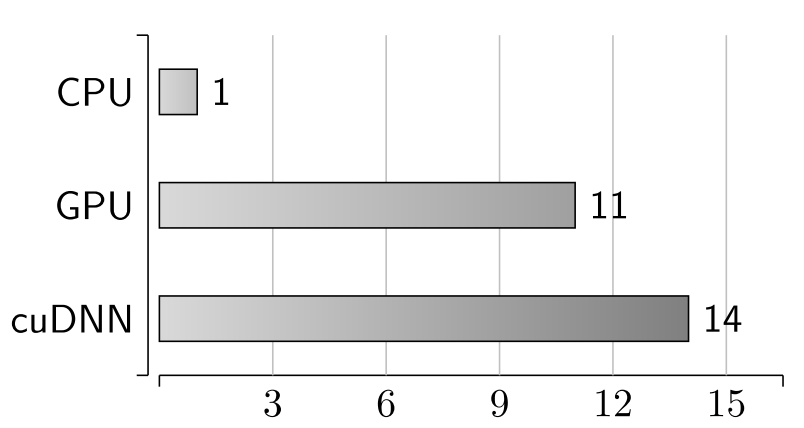
\includegraphics[width=0.5\textwidth]{figures/cpuvsgpu}
    \caption{ Neural network copmutation performance of different hardwares}
    \label{fig:cpuvsgpu}
\end{figure}

For the duration of the thesis, we gradually increase our access to more extensive learning resources. At the beginning of the project, we used our lab computer at Human-Brain-Project Lab that only had an Nvidia GeForce GTX-670, 31.2gb Ram. Since we did not need many computational resources in the beginning, GeForce GT-670 with 4gb ram was enough for us. As the computational requirements got higher, we migrated to use google cloud services. We received free google cloud credits from Roboy\footnote{\url{https://roboy.org/}} only for two months of usage. Enabling us to train larger networks in parallel with a more current graphics card Nvidia Tesla V100\footnote{\url{https://www.nvidia.com/en-us/data-center/v100/}}. Tesla V100 is designed for AI research. Thus it is more optimized compared to the GeForce series in terms of neural network training. After the free usage period had ended, we switched to the LRZ cloud framework. At LRZ, we continued to have a Tesla V100 with 368gb and 20VCPUs. 

The increase in the compute capability delivered a faster physics simulation. In return, the total training time got faster. Apart from the computational capacities, among the three different platform, LRZ provided the fastest internet connection. Having their server center at Garching, there was no recognizable latency. Although Google cloud platform servers are located in Frankurt, we suffered with a laggy internet connection. 
Overall LRZ cloud computation framework provides a safe and fast connection. Moreover, we received a quick response to our questions regarding the framework usage.

The remote desktop connection was a necessary tool for our project. Given that we trained neural networks entirely on the cloud, we needed a way to visualize the trained agents. Copying the trained model file back to the local computer is an option. Even though PyBullet supports MacOS, the neural network's forward pass still takes long on consumer hardware. For these reasons, we needed to use remote desktop connections. We tested two different remote desktop software: VNCViewer, and Tiger Remote Desktop. Tiger remote desktop has the edge over VNCViewer in terms of lightweight and user-friendly design. Besides, we often experienced blurred views and unable to change the screen resolution on VNCViewer. We installed the Xfce\footnote{\url{https://www.xfce.org/}} Unix based desktop environment on the LRZ cloud machine and forwarded the VNC port to localhost to connect with Tiger Remote Desktop. Xfce delivers a lightweight, easy-to-use desktop environment. We were overall satisfied with the performance of the remote desktop environment. 

\begin{figure}[htbp]
    \centering
    \begin{subfigure}{0.48\textwidth}
      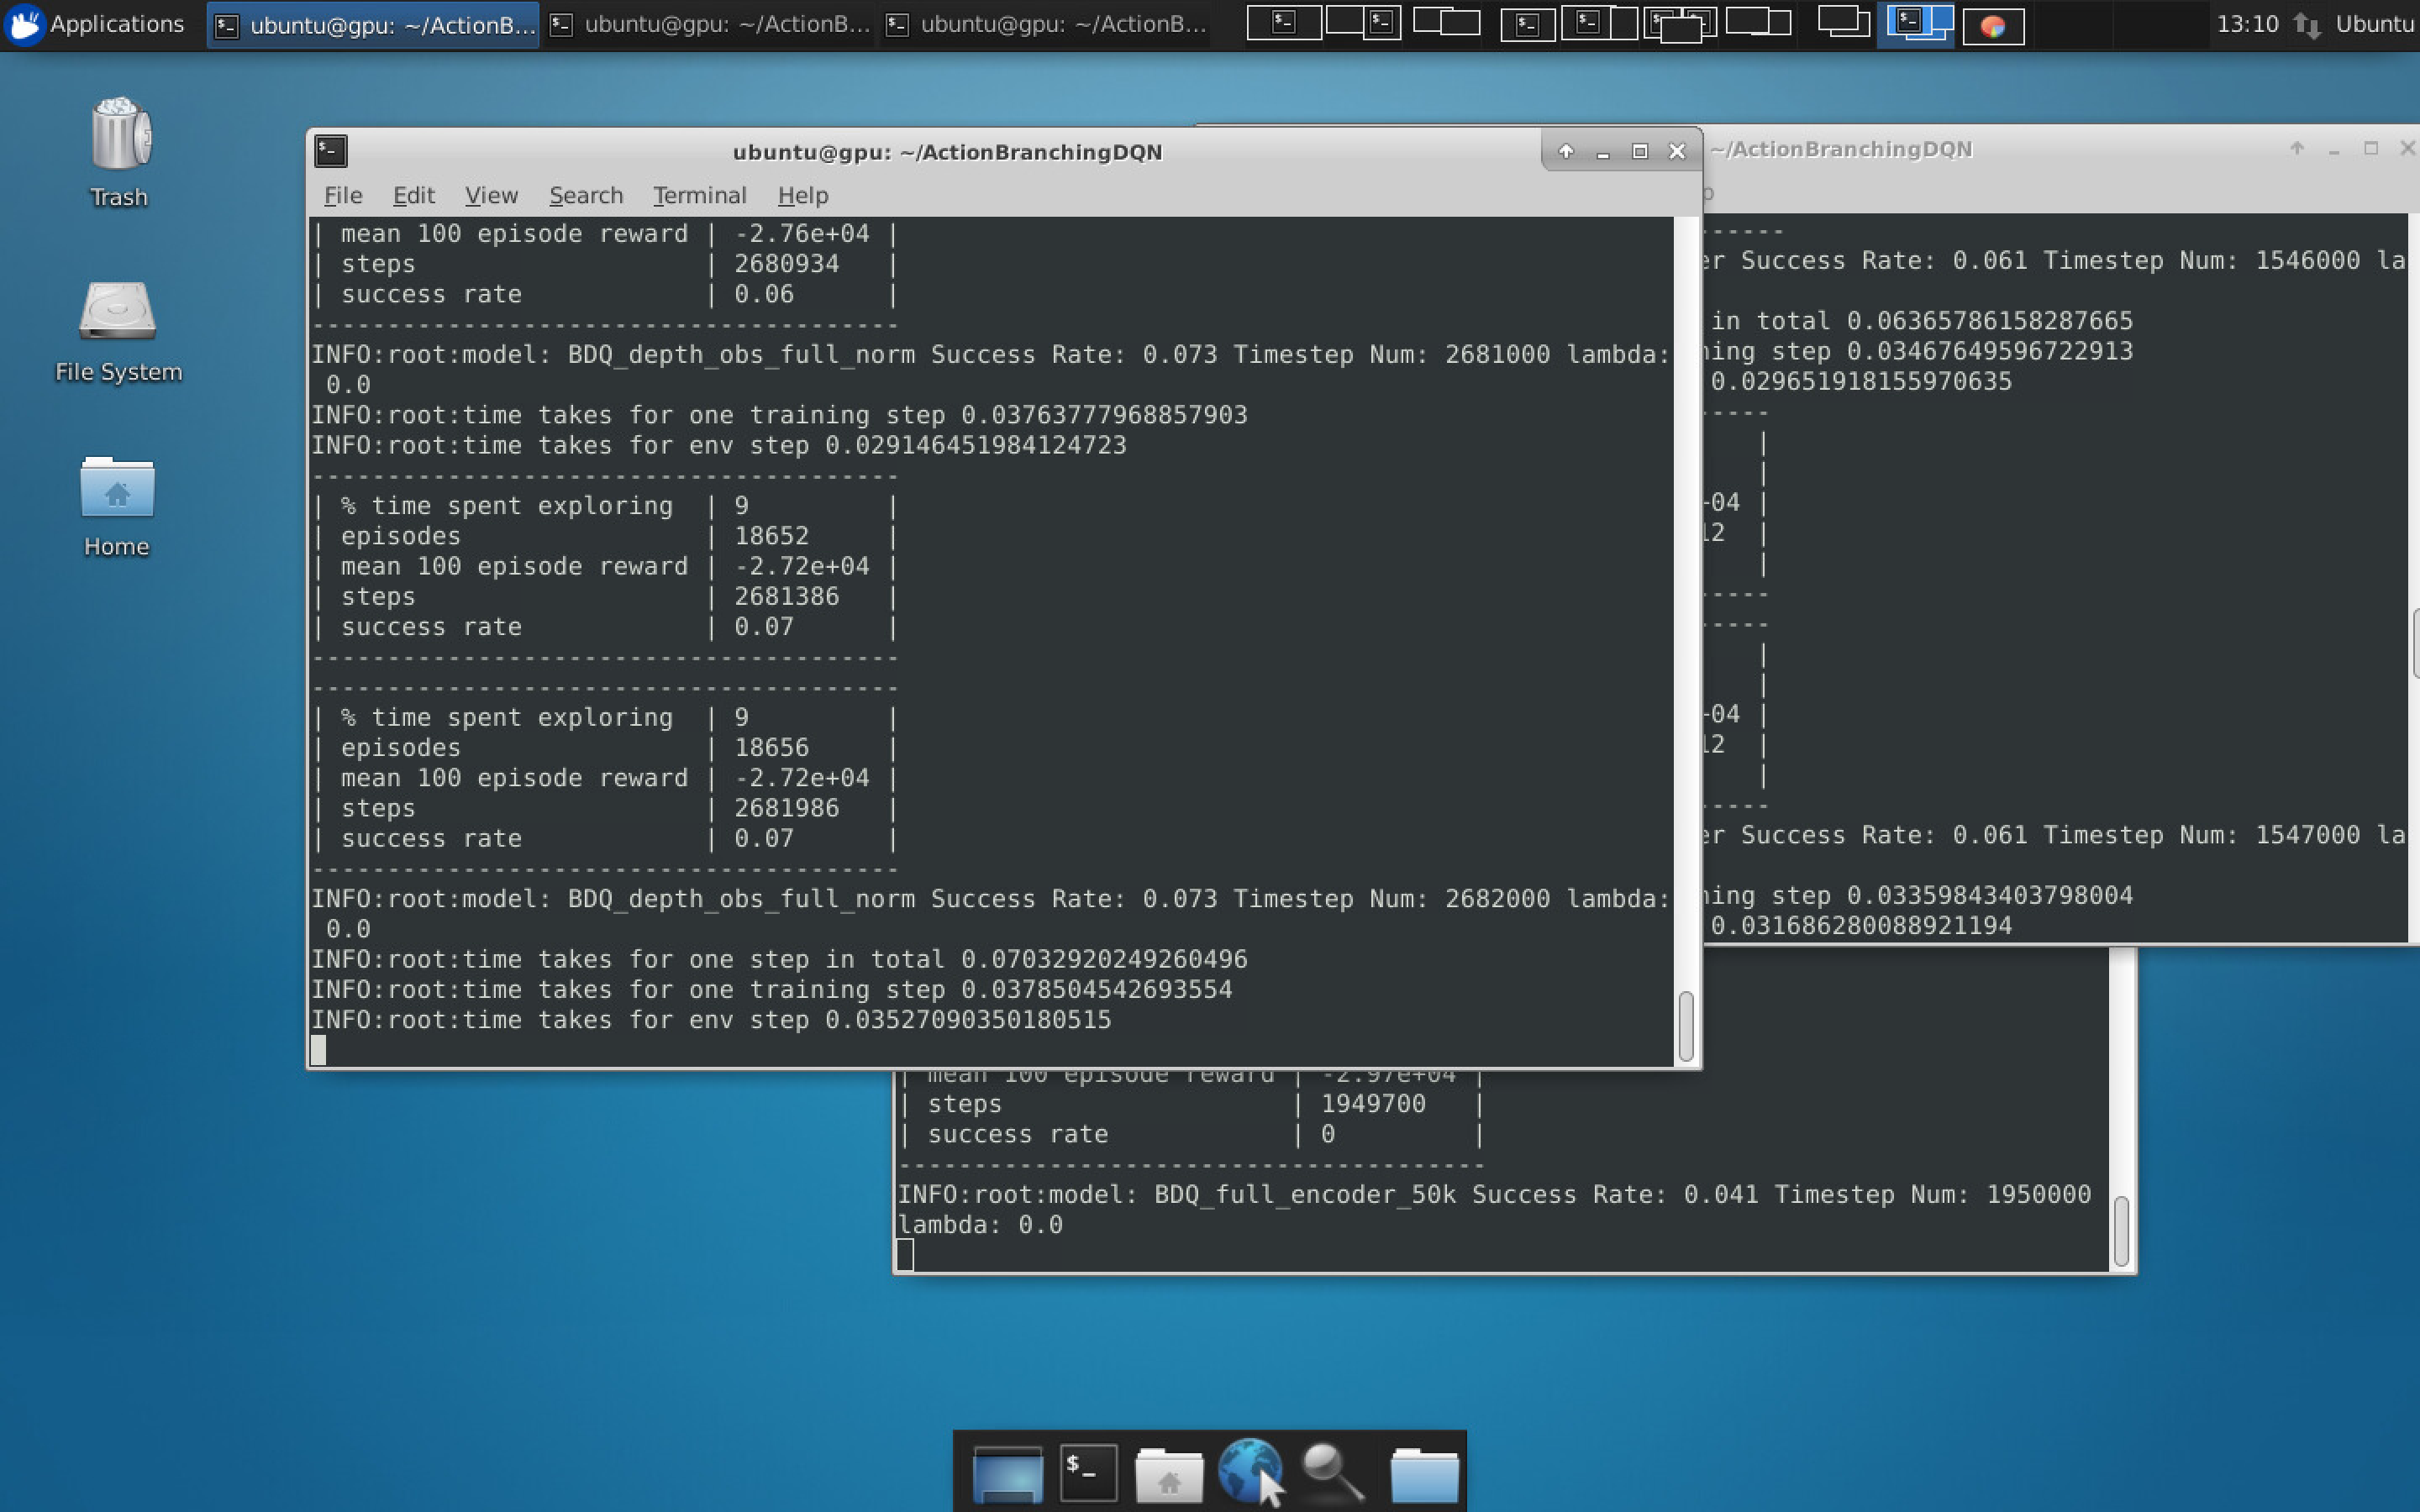
\includegraphics[width=1\linewidth]{figures/tiger}
      \caption{ Screenshot of Xfce desktop on LRZ cloud from Tiger remote desktop tool} \label{fig:tiger}
    \end{subfigure}%
    \hspace*{\fill}   % maximize separation between the subfigures
    \begin{subfigure}{0.48\textwidth}
      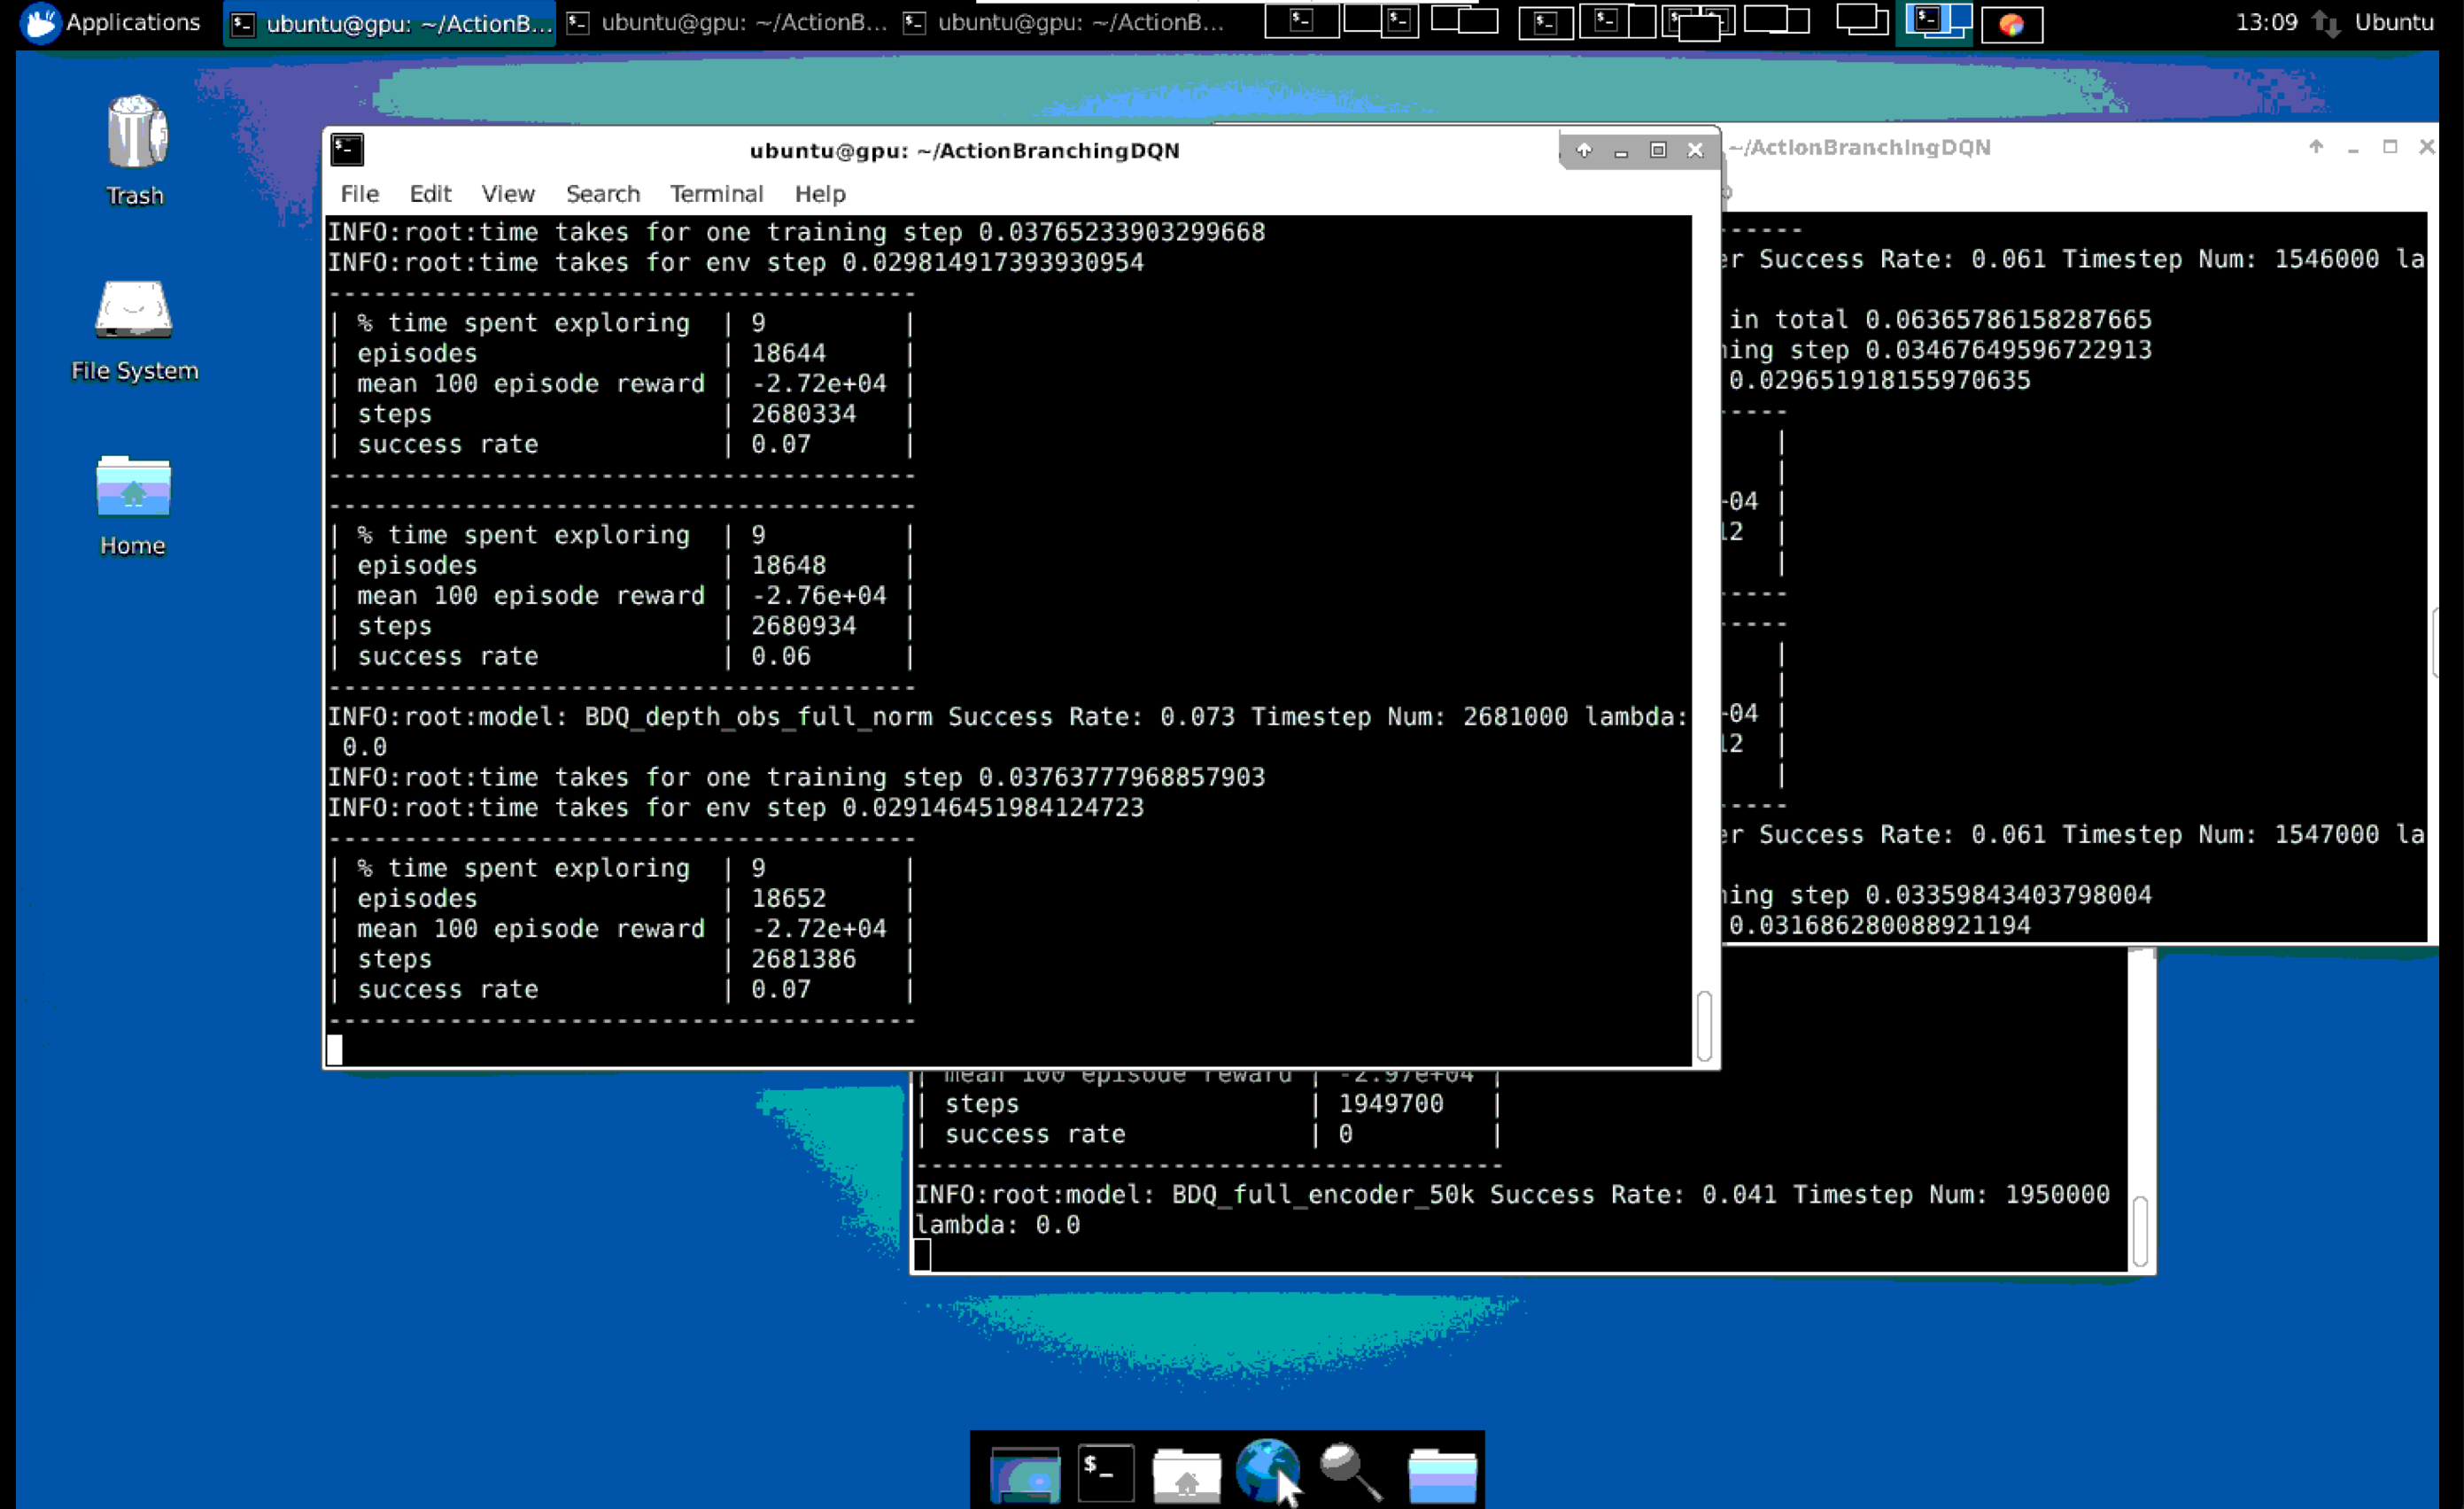
\includegraphics[width=1\linewidth]{figures/vncviewer}
      \caption{ Fuzzy view problem from VNCViewer remote desktop tool} \label{fig:vncviewer}
    \end{subfigure}%
    % \hspace*{\fill}   % maximize separation between the subfigures

\caption{ Remote desktop connection to LRZ cloud computing \label{fig:lrzcloud}}
\end{figure}